\section{Field Programmable Gate Arrays (FPGAs)}

A Field Programmable Gate Array (FPGA) is an integrated circuit designed to be configured; it consists of an array of programmable logic blocks and a hierarchy of reconfigurable interconnects. This architecture allows defining the hardware at the gate level, effectively creating a custom processor tailored to a specific algorithm.


In the context of Digital Signal Processing (DSP), the importance of FPGAs originates from their ability to exploit hardware-level parallelism. As noted by \cite[pp. 1--14]{FPGAbasedImplementationSignal2008}, many DSP algorithms such as Finite Impulse Response (FIR) filters, Fast Fourier Transforms (FFT), and matrix operations are inherently repetitive and computationally intensive. While a standard CPU would process these samples one by one, an FPGA can implement dedicated hardware pipelines that process multiple data points simultaneously. This results in significantly higher throughput and deterministic latency, which are critical requirements for real-time physics instrumentation and high-frequency data acquisition.



also talk about specific one used (arty z7-20) \cite{ArtyZ7Reference} and its relevant specs in the project like the ADC and maybe why it would be better to change it for an external one. Talk about the PS and PL logic

\subsection{Communication Interfaces}
Explain AXI protocols to understand a little bit why it is important to introduce an IP like the comblock or later a complete workflow with DMA, UDMA and HOG.

\subsection{Comblock}

The communication between the Processing System (PS) and the Programmable Logic (PL) is one of the most critical and time-consuming aspects of FPGA-based instrumentation design. While the Advanced eXtensible Interface (AXI) standard provides the necessary framework for this interaction, implementing custom AXI-compliant slaves from scratch requires deep knowledge of bus handshaking, address decoding, and timing constraints. To mitigate this complexity, the International Centre for Theoretical Physics (ICTP) developed the ComBlock (Communication Block) \cite{FilesMasterRodrigo2021}, an open-source IP core designed to act as a versatile and simplified interface between the Zynq SoC's ARM processor and the custom logic implemented in the FPGA.

The primary objective of the ComBlock is to provide a Hardware Abstraction Layer at the logic level. It reduces the effort in three fundamental ways:

\begin{itemize}
    \item \textbf{Encapsulation of AXI Protocols:} The ComBlock hides the complexity of the AXI4-Lite and AXI4-Full protocols. It provides a simple set of parallel input and output ports (registers, FIFOs and DRAM) that can be directly connected to VHDL.
    \item \textbf{Unified Register Mapping:} It provides a pre-configured register bank, illustrated in \cref{fig:comblock_schematic}, divided into Output Registers, which allow the PS to send control parameters to the PL, and Input Registers, which allow the PL to send status information back to the PS. This fixed structure eliminates the need for manual address mapping in Vivado.
\end{itemize}


\begin{figure}
    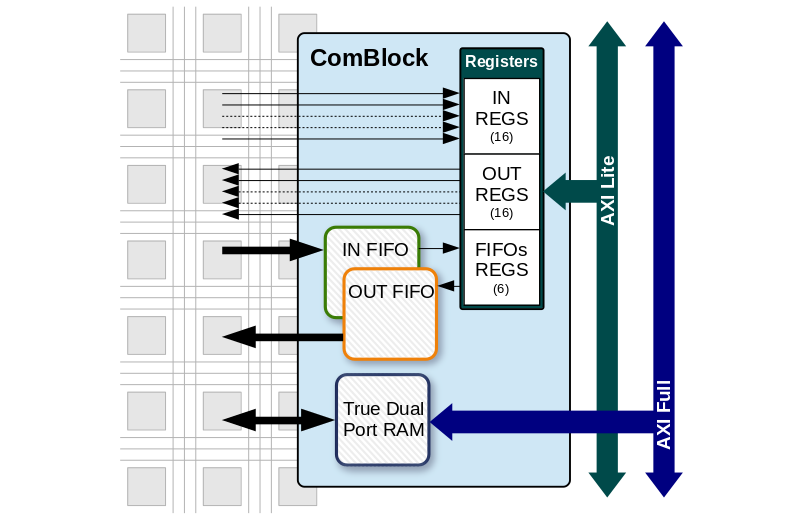
\includegraphics[width=12cm]{images/comblock.png}
    \caption{Comblock schematic taken from \cite{FilesMasterRodrigo2021}}
    \label{fig:comblock_schematic}
\end{figure}

The integration of the ComBlock into a Vivado design follows a Plug-and-Play methodology within the IP Integrator environment. Once added to the Block Design, the ComBlock is connected to the Zynq Processing System through the AXI Interconnect, this task can be done automatically with the Vivado-IDE functions.


\emph{maybe explain a little bit more in detail an example??}

\subsection{PYNQ}

The development of custom hardware on FPGAs has traditionally been governed by Hardware Description Languages (HDLs), such as VHDL and Verilog. Unlike high-level programming languages (C or Python) that follow a sequential execution model, HDLs are used to describe the concurrent behavior and structural connectivity of digital logic. This fundamental difference imposes a steep learning curve on researchers, as hardware design requires deep knowledge of digital electronics and clock domain crossing. The productivity gap in FPGA design originates from the fact that even minor changes in a digital circuit require a full synthesis and implementation cycle, which can take from several minutes to hours. Furthermore, interfacing the hardware logic with a host computer for data analysis usually involves writing drivers in C. To address these challenges, the PYNQ framework was introduced \cite{PYNQ}.

Hardware Description Languages and their high learning curve explain how PYNQ tries to solve this problem by simplifying its usage

\subsection{HOG}
How this framework reduces time and unifies hdl workflows in order to have a real collaborative environment on shared projects; also improving their replicability having in mind the open-hardware approach


\subsection{Comblock API for PYNQ}
Show the API created and the repo, how it simplifies the workflow and what good practices (HOG) are implemented for better usability. 